\begin{figure}[htbp]
\centering
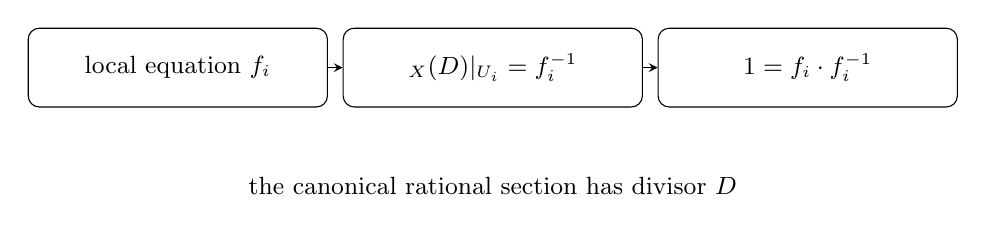
\begin{tikzpicture}[>=stealth,every node/.style={font=\small}]
\node[draw,rounded corners,minimum width=3.8cm,minimum height=1cm] (d) at (-4,0) {local equation $f_i$};
\node[draw,rounded corners,minimum width=3.8cm,minimum height=1cm] (o) at (0,0) {$\OO_X(D)|_{U_i}=f_i^{-1}\OO$};
\node[draw,rounded corners,minimum width=3.8cm,minimum height=1cm] (s) at (4,0) {$1=f_i\cdot f_i^{-1}$};
\draw[->] (d)--(o);
\draw[->] (o)--(s);
\node at (0,-1.5) {the canonical rational section has divisor $D$};
\end{tikzpicture}
\caption{A Cartier equation becomes the local coefficient of the canonical rational section of $\OO_X(D)$.}
\label{fig:vi40-oxd}
\end{figure}
